\chapter{Serwis społecznościowy Twitter}
Serwis spo\l{}eczno\'sciowy Twitter jest ameryka\'nskim serwisem internetowym s\l{}u\.z\k{a}cym g\l{}\'ownie do zamieszczania wiadomo\'sci tzw. "tweet\'ow", kt\'ore u\.zytkownicy tego serwisu mog\k{a} także: czytać, komentowa\'c lub przekazywa\'c dalej. Od kilku lat Twitter jest serwisem gdzie dochodzi do wymiany zdań na różny temat dotyczących np. polityki, sportu, produktów, wydarzeń społecznych, a profile posiada wiele osób znanych publicznie oraz instytucji.

\section{Historia}
Serwis ten, nazywany SMS internetu, zosta\l{} za\l{}o\.zony w 2006 r. w Stanach Zjednoczonych przez Jacka Dorseya, Ev Williamsa, Noah Glassa oraz Biza Stone’a i od początku swojego powstania sukcesywnie zwi\k{e}ksza\l{} swoj\k{a} popularno\'s\'c poprzez wzrost liczby u\.zytkownik\'ow odwiedzaj\k{a}cych jego witryn\k{e} oraz wysy\l{}aj\k{a}cych wiadomo\'sci. W 2012 r. osiągnął‚ ponad 100 milionów użytkowników, którzy zamieszczali łącznie ponad 340 milionów wiadomo\'sci dziennie wraz z obsługą \'srednio około 1.6 miliarda wyszukujących zapytań dziennie. W 2013 r. Twitter stał si\k{e} jedną z najcze\'sciej odwiedzanych stron w całym internecie. Inżynierowie Twittera podali informację w 2013 r., że serwis ten obsługuje ok. 143 tys. wiadomości na sekundę. Na początku 2016 r. serwis ten posiadał ponad 319 milionów użytkowników aktywnych podczas każdego miesiąca. Od listopada 2013 r. akcje Twittera są obecne na nowojorskiej giełdzie.

\section{Tweet}
Tweety, czyli krótkie wiadomości tekstowe, by\l{}y pocz\k{a}tkowo ograniczone do 140 znak\'ow, ale limit ten zosta\l{} podwojony w 2017 r. dla wszystkich j\k{e}zyk\'ow opr\'ocz chi\'nskiego, japo\'nskiego i korea\'nskiego. Użytkownicy mają możliwość wyróżniania wybranych przez siebie tematów przez dodanie do nich znaku '\#', co czyni takie wyrażenie tagiem. Inną możliwością oferowaną przez Twittera jest odpowiadanie innym użytkownikom lub zamieszczenie referencji do nich przez dodanie znaku '@' poprzedzającego nazwę profilu innej osoby.

\section{Architektura}
Serwis społecznościowy Twitter opierał się początkowo o typową architekturę trójwarstwową składająca się z warstwy prezentacji, logiki biznesowej oraz warstwy danych. Językiem programowania, w którym została napisana ta webowa aplikacja, był język Ruby on Rails, a warstwa bazodanowa opierała się o technologię MySQL. Jednak wraz ze wzrostem ilości przetwarzanych danych inżynierowie Twittera podjęli decyzję w 2011 r. o zmianie technologii na język Scala, który działa na maszynie wirtualnej Javy oraz zrezygnowano z dotychczasowej architektury na rzecz budowy rozproszonych serwisów komunikujących się między sobą. Wraz z przeprowadzonymi zmianami zanotowano ponad 10-krotne polepszenie obsługi tweetów.

\section{API}
Twitter jest platformą otwartą i udostępnia programowalny interfejs API w dwóch postaciach: Search API oraz Streaming API.

\subsection{Zakres działania}
Programiści korzystający z Search API są w stanie uzyskać dostęp tylko do danych historycznych, które zostały już wcześniej zamieszczone na łamach serwisu Twitter. Natomiast w przypadku Streaming API dostajemy możliwość śledzenia strumienia danych, które są do naszego dostępu nawet już kilka sekund po zamieszczeniu na łamach serwisu Twitter. Po podłączeniu do takiego strumienia możemy cały czas obserwować nowe wiadomości. Przyjęło się stosować nazywnictwo, że analiza Search API to analiza \textit{back in time}, a Streaming API to śledzenie \textit{real time}.

\subsection{Rejestracja}
Obie formy API wymagają wcześniej rejestracji na stronie \textit{https://developer.twitter.com/en/apply-for-access} przeznaczonej dla deweloperów zainteresowanych wykorzystywaniem Twitter API. Po przejściu pomyślnej rejestracji dostajemy dane, które po nawiązaniu połączenia z serwisem Twitter umożliwiają mu jednoznacznie określić, że możemy uzyskać dostęp do API.

\subsection{Sposób działania}
Search API powstało z wykorzystaniem standardu REST - \textit{Representational State Transfer}. Oba rodzaje API wykorzystują protokół HTTP: do poprawnego działania Streaming API potrzebne jest ciągłe połączenie HTTP, a w przypadku drugiego z nich każda operacja jest wykonywana przy nawiązaniu oddzielnego połaczenia.

\begin{figure}[h] % h means here
	\centering
	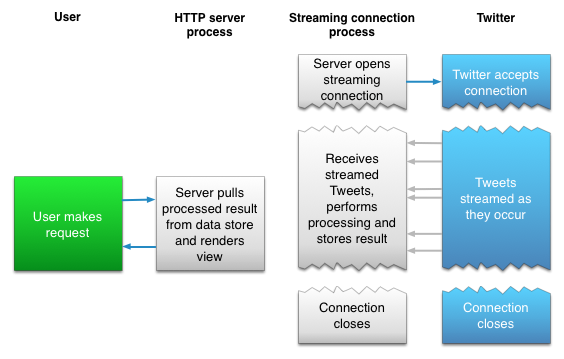
\includegraphics[width=0.6\linewidth]{img/twitter_api_comparison}
	\caption{Schemat działania dwóch rodzajów programistycznego interfejsu API udostępnianego przez serwis społecznościowy Twitter: Search API i Streaming API.}
\end{figure}

Search API posiada ściśle określone paramtery, które mogą być przesłane w żądaniu. Poniżej prezentuję ich wykaz.

\begin{table}
\centering
\caption{Parametry żądania \textit{Twitter Search API} [3].}
\label{tab:table1}
\begin{tabularx}{\linewidth}{|c|c|X|c|}\toprule
    Parametr & {Wymagany/Opcjonalny} & {Opis} & {Przykład} \\ \midrule
    q & wymagany & {zapytanie wyszukujące o maksymalnej długości 500 znaków} & nasa \\ \midrule
    geocode & opcjonalny & {zwraca wiadomości użytkowników oddalonych o podany promień od podanej szerokości i długości geograficznej, promień może być podany w milach lub kilometrach} & {37.781157 -122.398720 1mi} \\ \midrule
    lang & opcjonalny & {ogranicza wiadomości do wybranego języka spośród dostępnych kodów ISO 639-1} & {pl} \\ \midrule
    locale & opcjonalny & {specyfikuje język wysyłanego zapytania, obecnie tylko \textit ja jest skuteczny} & {ja} \\ \midrule
    result\textunderscore type & opcjonalny & {określa typ zwracanych wiadomości, obecnie dostępne są trzy wartości tego parametru: \textit{recent} (zwracane są najnowsze wiadomości), \textit{popular} (zwracane są najbardziej popularne wiadomości) \textit{mixed} (wartość domyślna, zwracane wyniki obejmują najnowsze i najbardziej popularne wiadomości)} & {mixed} \\ \midrule
    count & opcjonalny & {specyfikuje ilość zwracanych wiadomości; maksymalna wartość to 100, a domyślna to 15} & 100 \\ \midrule
\end{tabularx}
\end{table}


Streaming API nie posiada takich ograniczeń. W języku programowania Java dostępne są pakiety zawierające klasy \textit{User} oraz \textit{Status}, na które mapowane są przychodzące ze strumienia informacje. Poniżej zamieszczam ich dokumentację.

\begin{table}
\centering
\caption{Parametry żądania \textit{Twitter Search API} [3].}
\label{tab:table1}
\begin{tabularx}{\linewidth}{|c|c|X|c|}\toprule
    Parametr & {Wymagany/Opcjonalny} & {Opis} & {Przykład} \\ \midrule
    q & wymagany & {zapytanie wyszukujące o maksymalnej długości 500 znaków} & nasa \\ \midrule
    geocode & opcjonalny & {zwraca wiadomości użytkowników oddalonych o podany promień od podanej szerokości i długości geograficznej, promień może być podany w milach lub kilometrach} & {37.781157 -122.398720 1mi} \\ \midrule
    lang & opcjonalny & {ogranicza wiadomości do wybranego języka spośród dostępnych kodów ISO 639-1} & {pl} \\ \midrule
    locale & opcjonalny & {specyfikuje język wysyłanego zapytania, obecnie tylko \textit ja jest skuteczny} & {ja} \\ \midrule
    result\textunderscore type & opcjonalny & {określa typ zwracanych wiadomości, obecnie dostępne są trzy wartości tego parametru: \textit{recent} (zwracane są najnowsze wiadomości), \textit{popular} (zwracane są najbardziej popularne wiadomości) \textit{mixed} (wartość domyślna, zwracane wyniki obejmują najnowsze i najbardziej popularne wiadomości)} & {mixed} \\ \midrule
    count & opcjonalny & {specyfikuje ilość zwracanych wiadomości; maksymalna wartość to 100, a domyślna to 15} & 100 \\ \midrule
\end{tabularx}
\end{table}


\subsection{Ograniczenia}
Korzystając z Search API mamy możliwość wysłania 720 zapytań na godzinę, a maksymalna ilość wiadomości jaka może być zwrócona na jedno zapytanie to 100. Jeśli wykorzystalibyśmy ten limit w maksymalny sposób to daje nam to 72 000 wiadomości na godzinę. W przypadku Streaming API głównym ograniczeniem jest dostęp do ok. 1 \% danych ze strumienia, a maksymalna ilość wiadomości w czasie jednej minuty to 3 000. W przypadku tego API w ciągu godziny możemy uzyskać 180 000 wiadomości na godzinę. Są to ograniczenia, które obowiązują dla rozwiązań typu \textit{open-source}.

\section{Dostępne narzędzia analityczne}